\documentclass[11pt,a4paper]{article}
\usepackage[margin=2.4cm]{geometry}
\usepackage{amsmath,amssymb,graphicx,booktabs,hyperref,caption}
\usepackage{mathptmx}
\captionsetup{font=small,labelfont=bf}
\hypersetup{colorlinks=true,linkcolor=black,citecolor=black,urlcolor=blue}
% generated by paper/make_numbers.py - do not edit
\newcommand{\NHalos}{10}
\newcommand{\NPhases}{24}
\newcommand{\NSamples}{150}
\newcommand{\NLevels}{22}
\newcommand{\NTrajPerCurve}{79,200}
\newcommand{\NTrajTotal}{3,168,000}
\newcommand{\AzMin}{7,794}
\newcommand{\AzMax}{75,992}
\newcommand{\KMax}{588}
\newcommand{\KMin}{10.9}
\newcommand{\SposAFirst}{103}
\newcommand{\SposALast}{18,200}
\newcommand{\SposBFirst}{7.08}
\newcommand{\SposBLast}{n/a}
\newcommand{\SvelAFirst}{3.96}
\newcommand{\SvelALast}{185}
\newcommand{\SvelBFirst}{228}
\newcommand{\SvelBLast}{n/a}
\newcommand{\AzKnee}{62,353}
\newcommand{\KKnee}{71.7}
\newcommand{\SposAKnee}{1,410}
\newcommand{\SvelAKnee}{29.1}
\newcommand{\GainPosKnee}{14}
\newcommand{\SposALastKm}{18.2}
\newcommand{\NBOutOfRange}{2}
\newcommand{\SposBLastFinite}{189}
\newcommand{\AzBLastFinite}{62,353}
\newcommand{\SigMaxKm}{390}
\newcommand{\SigMaxMms}{1,020}
\newcommand{\GainPosA}{180}
\newcommand{\GainVelA}{47}
\newcommand{\RatioBA}{63--135}
\newcommand{\FitPosA}{-1.22}
\newcommand{\FitPosARms}{0.17}
\newcommand{\FitVelA}{-0.95}
\newcommand{\FitVelARms}{0.06}
\newcommand{\FitPosB}{-1.39}
\newcommand{\FitPosBRms}{0.18}
\newcommand{\FitVelB}{-0.70}
\newcommand{\FitVelBRms}{0.06}
\newcommand{\PNFlips}{11}
\newcommand{\PNTotal}{3,168,000}
\newcommand{\PNFlipFrac}{3.5\times10^{-6}}
\newcommand{\PNMaxDiff}{2.8\times10^{-4}}
\newcommand{\PNEquivMedMM}{1.6}
\newcommand{\PNEquivMaxMM}{5.8}
\newcommand{\PNShiftMed}{35}
\newcommand{\PNShiftMax}{1,800}
\newcommand{\PNRatioMed}{4.3\times10^{-11}}
\newcommand{\PNEquivOverTol}{1.8\times10^{-4}}
\newcommand{\RouteSpreadMin}{15}
\newcommand{\RouteSpreadMax}{990}
\newcommand{\BestRouteFirst}{585}
\newcommand{\BestRouteLast}{43,300}
\newcommand{\LinRatioMin}{1.08}
\newcommand{\LinRatioMax}{2.21}
\newcommand{\RouteLinMin}{0.56}
\newcommand{\RouteLinMax}{4.77}
\newcommand{\GainMin}{2.0\times10^{2}}
\newcommand{\GainMax}{5.1\times10^{6}}
\newcommand{\MidAz}{46,764}
\newcommand{\MidK}{199}
\newcommand{\NrevHalf}{10,100}
\newcommand{\NrevOne}{460}
\newcommand{\NrevOneHalf}{25.6}
\newcommand{\NrevTwo}{1.18}
\newcommand{\ScanUsableMin}{71}
\newcommand{\ScanUsableMax}{100}
\newcommand{\ConvRel}{1.3\times10^{-3}}
\newcommand{\FamilySize}{283}
\newcommand{\FlightMin}{2.3}
\newcommand{\FlightMax}{12.0}
\newcommand{\ResultRows}{%
7,794 & 15.13 & 3.1624 & 588 & 103 (59--150) & 7.08 & 3.96 & 228 \\
15,588 & 15.08 & 3.1572 & 537 & 141 (82--210) & 9.05 & 4.51 & 217 \\
23,382 & 15.01 & 3.1489 & 462 & 197 (120--270) & 14.6 & 5.47 & 247 \\
31,176 & 14.90 & 3.1378 & 373 & 284 (190--400) & 20.9 & 6.89 & 266 \\
38,970 & 14.75 & 3.1242 & 283 & 402 (240--580) & 25.3 & 8.85 & 336 \\
46,764 & 14.55 & 3.1084 & 199 & 460 (260--780) & 34.4 & 11 & 423 \\
54,558 & 14.27 & 3.0909 & 127 & 656 (370--1,200) & 55.6 & 16.1 & 654 \\
62,353 & 13.87 & 3.0717 & 71.7 & 1,410 (860--2,300) & 189 & 29.1 & $>$1,020 \\
70,147 & 13.20 & 3.0512 & 31.9 & 5,060 (3,300--7,600) & $>$390 & 69.2 & $>$1,020 \\
75,992 & 12.21 & 3.0350 & 10.9 & 18,200 (14,000--22,000) & $>$390 & 185 & $>$1,020 \\
}
\newcommand{\RobustRows}{%
15,588 & 141 (82--210) & 143 & 65/79,200 & 134 & 130 & 35.3 & 551 \\
38,970 & 402 (240--580) & 404 & 36/79,200 & 367 & 388 & 99.6 & 1,550 \\
62,353 & 1,410 (860--2,300) & 1,410 & 29/79,200 & 1,360 & 1,650 & 365 & 5,290 \\
}
\newcommand{\DenseRows}{%
15,588 & 35 & 124 (79--190) & 127 (84--190) & 97.7 \\
38,970 & 39 & 404 (280--560) & 399 (280--530) & 313 \\
62,353 & 48 & 1,530 (1,000--2,200) & 1,510 (1,100--2,100) & 1,110 \\
}

\newcommand{\mum}{\mu}
\title{How much injection error can stable-manifold capture into an Earth--Moon L$_2$ halo orbit absorb?\\[4pt]
\large A Monte Carlo study in the circular restricted three-body problem, with a first post-Newtonian check}
\author{Shaurya\thanks{Independent student researcher. \textbf{Draft.} Code, data and the one-command reproduction script accompany this paper.}}
\date{Draft of \today}
\begin{document}
\maketitle

\begin{abstract}
\noindent A spacecraft placed exactly on the stable manifold of a halo orbit coasts into that orbit without
fuel. Real injections are never exact. For the northern Earth--Moon L$_2$ halo family in the circular
restricted three-body problem, I measure how large a Gaussian position or velocity error at injection can be
before an uncorrected spacecraft fails to be captured, and how that tolerance scales with orbit size.
Ten family members with out-of-plane amplitudes from \AzMin\ to \AzMax~km (stability index $k$ from \KMax\ down to \KMin) are studied with
\NTrajTotal\ trajectories. If capture means staying within 5000~km of the halo for one revolution, the
error at which half the spacecraft are captured rises from \SposAFirst~m for the smallest halo to \SposALastKm~km for the largest in position, and from
\SvelAFirst\ to \SvelALast~mm/s in velocity; against the stability index it scales roughly as $k^{\FitPosA}$ and $k^{\FitVelA}$ respectively.
Under a looser definition (remaining within two Hill radii of the Moon) the position tolerance is
\SposBFirst~km for the smallest halo and exceeds the largest error tested (\SigMaxKm~km) for the \NBOutOfRange\ largest.
The tolerance depends even more strongly on \emph{which} manifold trajectory is flown than on the halo:
routes that pass close to the Moon are up to \RouteSpreadMax\ times less forgiving. A linear prediction from the state transition matrix
reproduces the simulated per-route tolerances over four decades (ratios between \RouteLinMin\ and \RouteLinMax). Adding the first post-Newtonian (Einstein--Infeld--Hoffmann)
acceleration, of relative size \(\PNRatioMed\), changes \PNFlips\ of \PNTotal\ outcome classifications. The model omits the Sun, lunar
eccentricity and correction manoeuvres; the results describe how sensitivity scales, and are not a mission design.
\end{abstract}

\section{Introduction}
Halo orbits about the Earth--Moon L$_2$ point keep a spacecraft in view of both the Earth and the lunar far
side, and their near-rectilinear relatives are the planned home of the lunar Gateway. They are unstable, and
with that instability come invariant manifolds: families of trajectories that approach the orbit
asymptotically (stable manifold) or leave it (unstable manifold). A spacecraft on the stable manifold arrives
without an insertion burn, the basis of low-energy and ballistic-capture transfers \cite{koon}.

Because the destination is unstable, the same dynamics that carries a perfect spacecraft in also magnifies
any injection error. This paper asks a narrow, quantitative question:
\begin{quote}
For an Earth--Moon L$_2$ halo orbit, how large an injection error (position and velocity) can a spacecraft
absorb before stable-manifold capture fails, and how does that tolerance scale with orbit amplitude?
\end{quote}
The answer depends on what ``capture'' means, so two definitions are carried through the whole study. A
secondary question is whether general-relativistic corrections matter at this level.

\section{Model, assumptions and what they cost}\label{sec:model}
\paragraph{Circular restricted three-body problem (CR3BP).} Earth and Moon move on circles about their
barycentre; the spacecraft has negligible mass. In the frame rotating with the primaries, with the
Earth--Moon distance, the total mass and the inverse mean motion as units, the equations of motion are
\cite{koon,szebehely}
\begin{equation}
\ddot x-2\dot y=\Omega_x,\qquad \ddot y+2\dot x=\Omega_y,\qquad \ddot z=\Omega_z,\qquad
\Omega=\tfrac12(x^2+y^2)+\frac{1-\mum}{r_1}+\frac{\mum}{r_2}+\tfrac12\mum(1-\mum),
\end{equation}
with $r_1,r_2$ the distances to Earth at $(-\mum,0,0)$ and Moon at $(1-\mum,0,0)$. The terms of $\Omega$ are the
centrifugal potential and the two gravitational potentials; $-2\dot y$, $+2\dot x$ are the Coriolis
acceleration. I use $\mum=0.01215058560962404$, a length unit of 389\,703.26~km and a time unit of
382\,981.29~s, the values of NASA/JPL's periodic-orbit catalogue \cite{jplapi}, so that published orbits can
be reproduced exactly. The Jacobi constant $C=2\Omega-v^2$ is conserved. (JPL's catalogue omits the
constant term of $\Omega$; its $C$ is smaller than the one used here by $\mum(1-\mum)=0.012003$.)

\paragraph{What the model leaves out, and the consequence.}
\begin{itemize}\setlength\itemsep{1pt}
\item \emph{The Sun.} Solar gravity perturbs Earth--Moon libration-point orbits noticeably over a month. Real
halos are quasi-periodic, and real manifolds are those of the perturbed orbit. Absolute tolerances here are therefore indicative only.
\item \emph{Lunar eccentricity} ($e\approx0.055$). The true problem is time-dependent; periodic orbits of the CR3BP
do not survive unchanged.
\item \emph{Non-spherical gravity} (lunar $J_2$ and higher). This matters mainly for the routes that pass within a few lunar radii,
which are also the least tolerant routes.
\item \emph{No correction manoeuvres.} Real missions correct every few days. ``Tolerance'' here means the error an
\emph{uncorrected} spacecraft survives, which is deliberately pessimistic; it is best read as how accurate
navigation must be until the first correction.
\item \emph{Gaussian, isotropic, uncorrelated errors.} Real injection errors are correlated and anisotropic (burn-direction
errors dominate).
\end{itemize}
None of these change the qualitative mechanism (exponential growth of the unstable component), but each could
change the numbers by factors of order one or more. Nothing here designs a real mission.

\section{Methods}
All computation is done by an open Python core; every number and figure in this paper is regenerated by one
command (Section~\ref{sec:repro}).

\subsection{Equilibria and their stability}
The collinear points are roots of $\Omega_x=0$ on the $x$ axis; L$_4$, L$_5$ are the equilateral points.
Linear stability follows from the eigenvalues of the $6\times6$ Jacobian of the flow. At L$_2$ the model gives
one real pair $\pm\lambda$ and two imaginary pairs $\pm i\nu$, $\pm i\omega_z$ with
$\lambda=2.1587$, $\nu=1.8626$, $\omega_z=1.7862$ (saddle $\times$ centre $\times$ centre).
Figure~\ref{fig:hill} shows the points and the regions forbidden by the Jacobi constant.

\begin{figure}[t]\centering
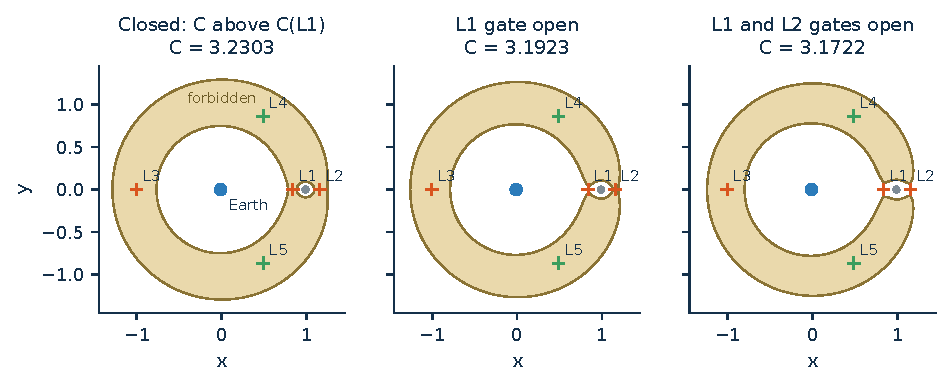
\includegraphics[width=\linewidth]{figures/fig1_hill_regions.pdf}
\caption{Lagrange points and Hill regions of the Earth--Moon CR3BP in the plane $z=0$. Shaded: forbidden at the
stated Jacobi constant. Lowering $C$ opens a gate first at L$_1$, then at L$_2$.}\label{fig:hill}
\end{figure}

\subsection{Halo orbits}
A third-order analytic approximation \cite{richardson} gives a first guess. It is refined by differential
correction that exploits the symmetry $(x,y,z,t)\to(x,-y,z,-t)$ \cite{howell}: an orbit that crosses the
$xz$ plane perpendicularly twice is periodic. With unknowns $X=(x_0,z_0,\dot y_0,\tau)$ and conditions
$F(X)=(y,\dot x,\dot z)|_{t=\tau}=0$, Newton's method uses the state transition matrix $\Phi$ (the solution of
$\dot\Phi=A(t)\Phi$, integrated as 36 extra equations) for the derivative of $F$. The one-parameter family is
followed by pseudo-arclength continuation, which is needed because the family turns back in $z_0$. The
monodromy matrix $M=\Phi(T)$ gives the Floquet multipliers; with $\lambda_u$ the largest in modulus, the
stability index is $k=\tfrac12(\lambda_u+1/\lambda_u)$.

\subsection{Invariant manifolds and the capture curve}
At each of $N$ evenly spaced phases $\phi$ of the orbit the stable eigenvector of $M$ is transported by $\Phi$ and
the state is displaced along it and integrated backwards. The displacement is
$\epsilon\,|p(\phi)|/\max|p|$ with $\epsilon=10^{-6}$ (at most 390~m), where $p(\phi)=\Phi(\phi T,0)\,v_s\,\lambda_s^{-\phi}$ is the
Floquet-periodic eigenvector and $|\cdot|$ its position length. This gives every start the same Floquet amplitude, so that the starts are
spread evenly over the trajectories of the tube; a constant displacement does not (Section~\ref{sec:pitfall}).
The Moon-bound branch is cut at its first crossing of the plane through the Moon, $x=1-\mum$. The set of
crossings is a closed curve in the four section coordinates (Fig.~\ref{fig:man}); I call it the capture curve.
Repeating with $\epsilon/10$ moves the curve by at most \(\ConvRel\) of its extent.

\subsection{Injection-error experiment}\label{sec:exp}
\emph{Nominal injection states.} For each halo, \NPhases\ points of the capture curve, spread around the tube.
Manifold trajectories that strike the Moon before the section, or whose \emph{unperturbed} forward flight does
not then hold the halo for two periods (they graze the Moon and amplify even rounding error), are excluded;
between \ScanUsableMin\% and \ScanUsableMax\% of scanned trajectories were usable, depending on the halo. This is a selection effect:
the results describe usable routes.

\emph{Errors.} Independent Gaussian errors per axis, either in position (standard deviation $\sigma_r$) or in
velocity ($\sigma_v$), at \NLevels\ logarithmically spaced levels from $10^{-10}$ to $10^{-3}$ non-dimensional
units (0.04~m to 390~km; $10^{-4}$~mm/s to 1~m/s). \NSamples\ draws are used and the \emph{same} draws are reused
at every level, for every halo and for every model (common random numbers), so differences between curves are
not sampling noise.

\emph{Propagation.} No manoeuvres. Dormand--Prince 8(5,3) with relative tolerance $10^{-12}$ and a step cap of
0.01 time units.

\emph{Classification.} With $T$ the halo period and $t_e$ the time at which the nominal trajectory first comes
within $d_{\rm tol}$ of the halo:
\begin{itemize}\setlength\itemsep{1pt}
\item[\textbf{A}] (halo-tracking) captured if the spacecraft stays within $d_{\rm tol}=5000$~km of the halo
for at least one consecutive period;
\item[\textbf{B}] (Moon-region) captured if it stays within two Hill radii of the Moon (124\,000~km) and does
not impact, until $t_e+T$.
\end{itemize}
Otherwise the outcome is \emph{impacted} (it reached the lunar or terrestrial surface first) or \emph{escaped}.
The summary statistic is $\sigma_{50}$, the error at which the pooled capture fraction crosses one half;
intervals are 16--84\% bootstrap ranges over draws and routes. With only \NPhases\ routes these ranges under-represent the spread of route sensitivities; Section~\ref{sec:robust} adds an all-routes check.

\emph{Linear prediction.} If $g$ is the largest singular value of the position rows of $\Phi(t_e+T,0)$ restricted to position
(or velocity) errors, an error is stretched to about $g\,|\xi|\sigma$ with $\xi$ standard normal, and capture
requires this to stay below $d_{\rm tol}$, so
\begin{equation}\label{eq:lin}\sigma_{50}\approx \frac{d_{\rm tol}}{0.674\,g}.\end{equation}

\subsection{First post-Newtonian correction}
The Einstein--Infeld--Hoffmann equations \cite{eih}, in the form used for planetary ephemerides
\cite{assist}, are implemented for $N$ bodies and, for the CR3BP, in the test-particle limit with the primaries
on their Newtonian circle (their own correction only alters the separation--period relation at the $10^{-11}$
level, absorbed by using observed units). The speed of light is $2.946\times10^{5}$ velocity units. The whole
experiment is repeated with this term, with the same random draws, the same nominal states and the same
Newtonian reference halo, i.e.\ without re-designing the orbit in the relativistic model, which is the pessimistic case.

\subsection{Verification}\label{sec:verif}
Automated checks, all passing (the accompanying verification report lists the measured values):
(i) with $\mum=0$ a circular orbit keeps its radius to $10^{-12}$ and an ellipse closes after one Kepler period;
(ii) a particle at L$_4$ moves less than $10^{-11}$ in 100 time units;
(iii) $x_{L_1}=0.836915$, $x_{L_2}=1.155682$, $x_{L_3}=-1.005063$, agreeing with \cite{jplapi} to 13 digits for L$_1$, L$_2$;
(iv) a $10^{-8}$ displacement at L$_1$ grows at a fitted rate within 0.2\% of $\lambda=2.9321$;
(v) relative Jacobi drift below $10^{-11}$ over multi-revolution runs;
(vi) three halos of \cite{jplapi}, including a near-rectilinear one, are reproduced from the analytic seed with
only $z_0$ taken from the catalogue: $x_0$, $\dot y_0$, $T$ and $C$ agree to better than $10^{-7}$ and $k$ to $10^{-4}$ (Fig.~\ref{fig:fam});
(vii) Mercury's perihelion advance from direct 1PN integration is 42.98$''$ per century and zero with the term off;
(viii) the Schwarzschild innermost stable circular orbit is found numerically at $6.000000\,GM/c^2$ and light
deflection at the solar limb is 1.751$''$;
(ix) the GPS clock offset is $+38.58~\mu$s per day ($4.4647\times10^{-10}$, as in \cite{ashby});
(x) halving every tolerance changes no conclusion (Section~\ref{sec:robust}).

\section{Results}
\subsection{The halo family}
The continuation produced \FamilySize\ members from the planar bifurcation to near-rectilinear orbits
(Fig.~\ref{fig:fam}). The stability index falls monotonically along the classic part of the family, from about 600
for the smallest halos to 1 where the family becomes linearly stable. Ten members with far-side crossing height
$z_0=0.02,\dots,0.195$ are used below; their amplitudes, periods and stability indices are in Table~\ref{tab:res}.

\begin{figure}[t]\centering
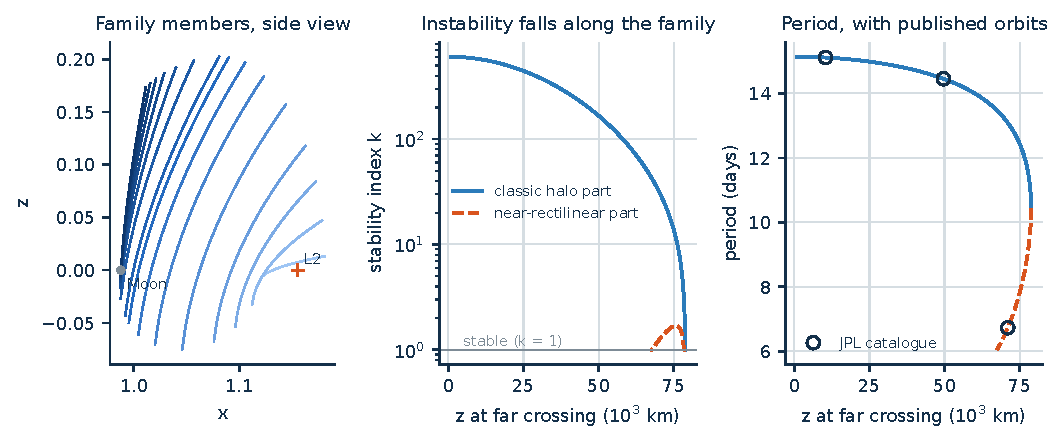
\includegraphics[width=\linewidth]{figures/fig2_halo_family.pdf}
\caption{Northern L$_2$ halo family. Left: members in the $xz$ plane (darker = further along the family).
Centre: stability index. Right: period, with three orbits from the JPL catalogue (circles) that this code reproduces.}\label{fig:fam}
\end{figure}

\begin{figure}[t]\centering
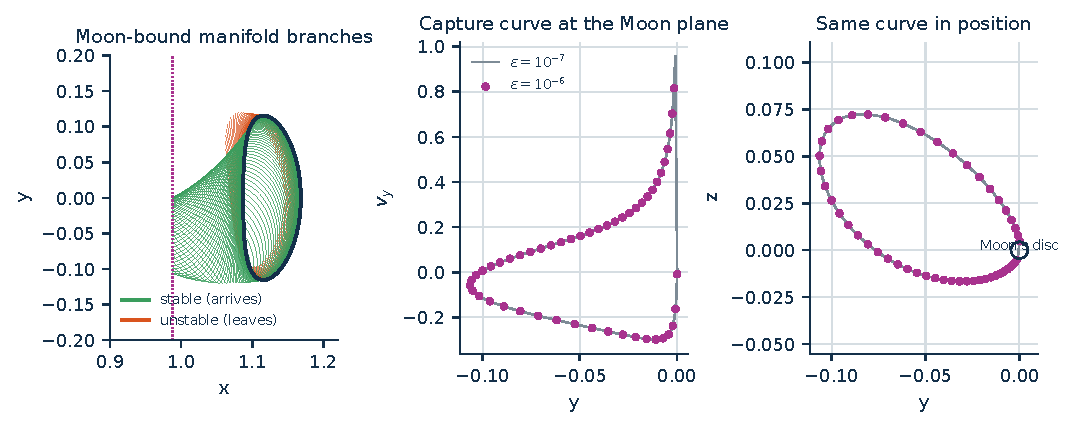
\includegraphics[width=\linewidth]{figures/fig3_manifolds.pdf}
\caption{Left: Moon-bound branches of the stable (green) and unstable (orange) manifolds of the halo with
$z_0=0.10$, in the rotating frame; the dotted line is the Moon plane. Centre, right: the capture curve where
the stable manifold meets that plane, for two values of the displacement $\epsilon$.}\label{fig:man}
\end{figure}

\subsection{Capture probability}
Figures~\ref{fig:pos} and \ref{fig:vel} show the capture fraction against error size. Each curve pools
\NTrajPerCurve\ trajectories. The curves are much wider than a single error function because they mix routes with very
different sensitivities (Section~\ref{sec:routes}). Larger halos tolerate larger errors under both definitions (colour runs from the smallest halo, lightest, to the largest, darkest).
Definition~B is far more forgiving, and its curves do not fall to zero at large errors: a spacecraft thrown far off
the manifold can still linger near the Moon for a month by chance, which definition~B counts.

\begin{figure}[t]\centering
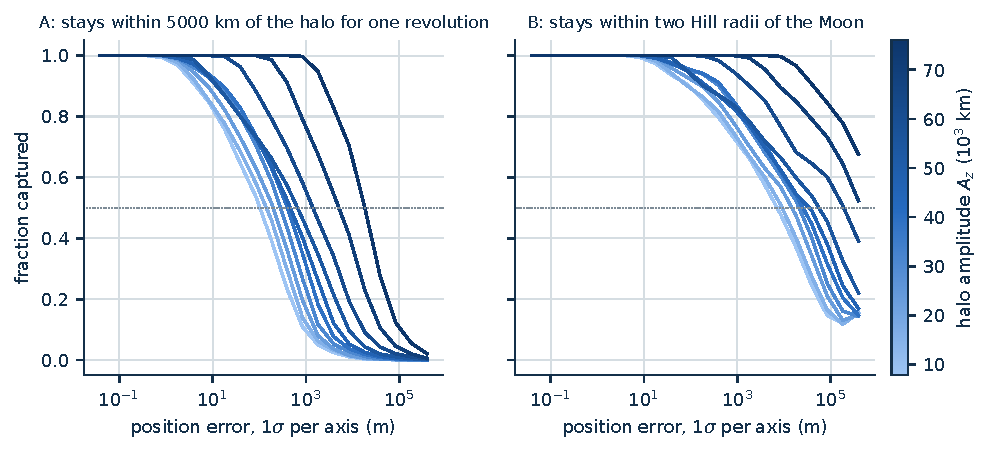
\includegraphics[width=\linewidth]{figures/fig4_capture_position.pdf}
\caption{Fraction captured against position error (velocity error zero) for the ten halos, under the two
definitions of capture.}\label{fig:pos}
\end{figure}
\begin{figure}[t]\centering
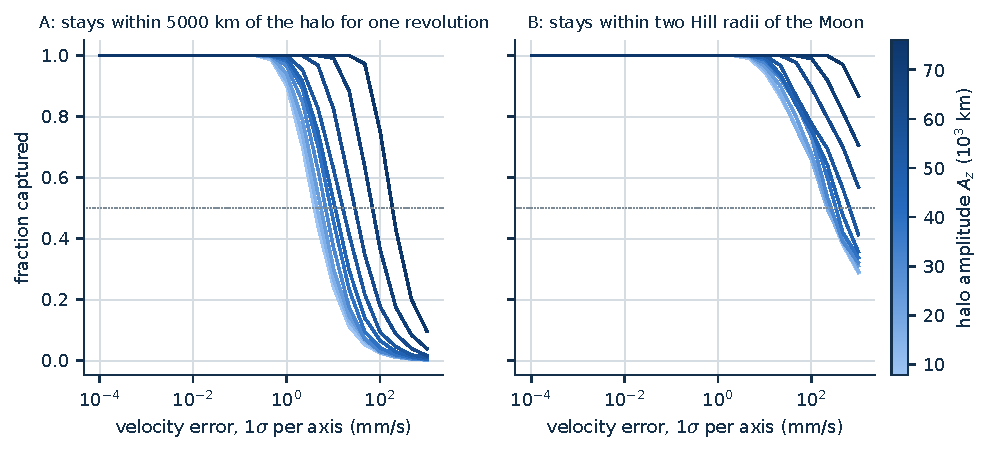
\includegraphics[width=\linewidth]{figures/fig5_capture_velocity.pdf}
\caption{As Fig.~\ref{fig:pos} for velocity error (position error zero).}\label{fig:vel}
\end{figure}

\begin{table}[t]\centering\small
\caption{Halos studied and 50\% capture tolerances. $A_z$: largest $|z|$. Brackets: 16--84\% bootstrap range.
A: halo-tracking; B: Moon-region.}\label{tab:res}
\begin{tabular}{rrrrrrrr}\toprule
$A_z$ & $T$ & $C$ & $k$ & $\sigma_{50}$ position, A & position, B & velocity, A & velocity, B\\
(km) & (d) & & & (m) & (km) & (mm/s) & (mm/s)\\\midrule
\ResultRows
\bottomrule\end{tabular}
\end{table}

\subsection{Scaling with amplitude and stability}
Under definition~A the position tolerance grows monotonically from \SposAFirst~m at $A_z=\AzMin$~km ($k=\KMax$) to \SposALastKm~km at
\AzMax~km ($k=\KMin$), a factor \GainPosA; the velocity tolerance grows from \SvelAFirst\ to \SvelALast~mm/s (factor \GainVelA).
Against the stability index both are close to power laws over this range (Fig.~\ref{fig:scale}, right):
$\sigma_{50}\propto k^{\FitPosA}$ in position (r.m.s.\ scatter \FitPosARms\ in $\ln\sigma_{50}$) and $k^{\FitVelA}$ in velocity (\FitVelARms).
An exponent near $-1$ is what growth by the factor $\lambda_u\approx2k$ during the required revolution would give. The position exponent is steeper,
plausibly because errors also grow along the approach leg, at a rate that weakens as $k$ falls; this explanation was not tested separately.
The linear prediction, Eq.~\eqref{eq:lin} averaged over routes, gives pooled tolerances within a factor
\LinRatioMin--\LinRatioMax\ of the simulation for every halo.
Under definition~B the tolerances are \RatioBA\ times larger where they could be measured; for the \NBOutOfRange\ largest halos more than half the
spacecraft remained near the Moon even at the largest error tested (\SigMaxKm~km in position), so only a lower bound can be given.

\begin{figure}[t]\centering
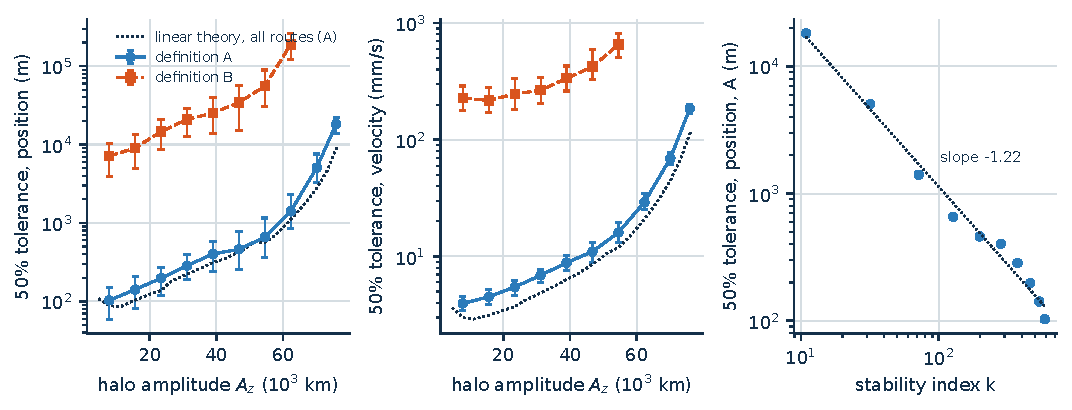
\includegraphics[width=\linewidth]{figures/fig6_tolerance_scaling.pdf}
\caption{50\% tolerance against halo amplitude for position (left) and velocity (centre) errors; bars are
bootstrap ranges; the dotted curve is the linear prediction for definition~A over all usable routes of a finer scan (24 halos). Right: position tolerance (A) against stability
index with the fitted power law. Definition~B points are missing where the capture fraction never fell to one half within the tested range.}\label{fig:scale}
\end{figure}

\subsection{The route matters more than the halo}\label{sec:routes}
For a single halo, $\sigma_{50}$ differs between injection points by factors of \RouteSpreadMin\ to \RouteSpreadMax\
(Fig.~\ref{fig:route}, left). The least tolerant routes are those whose manifold trajectory passes closest to the Moon,
where a small error is converted into a large change of direction. The linear growth factor $g$ ranges from \(\GainMin\) to \(\GainMax\) and
orders the routes almost perfectly: per-route tolerances follow Eq.~\eqref{eq:lin} within a factor \RouteLinMin--\RouteLinMax\
over four decades (Fig.~\ref{fig:route}, centre). The practical reading is that a designer gains more by choosing the arrival
route than by choosing the halo: on the best route the position tolerance is \BestRouteFirst~m for the smallest halo
and \BestRouteLast~m for the largest. Nominal coast times from injection to arrival are \FlightMin--\FlightMax~days.

The required dwell also matters greatly. For the halo with $A_z=\MidAz$~km ($k=\MidK$), requiring
$\tfrac12$, $1$, $1\tfrac12$ and $2$ revolutions gives $\sigma_{50}=$ \NrevHalf, \NrevOne, \NrevOneHalf\ and \NrevTwo~m:
every extra half revolution costs a factor of roughly $\sqrt{2k}$. When position and velocity errors act together, the 50\% contour is nearly rectangular (Fig.~\ref{fig:route}, right): capture
is lost when either error alone reaches its own tolerance, with little trade-off between them.

\begin{figure}[t]\centering
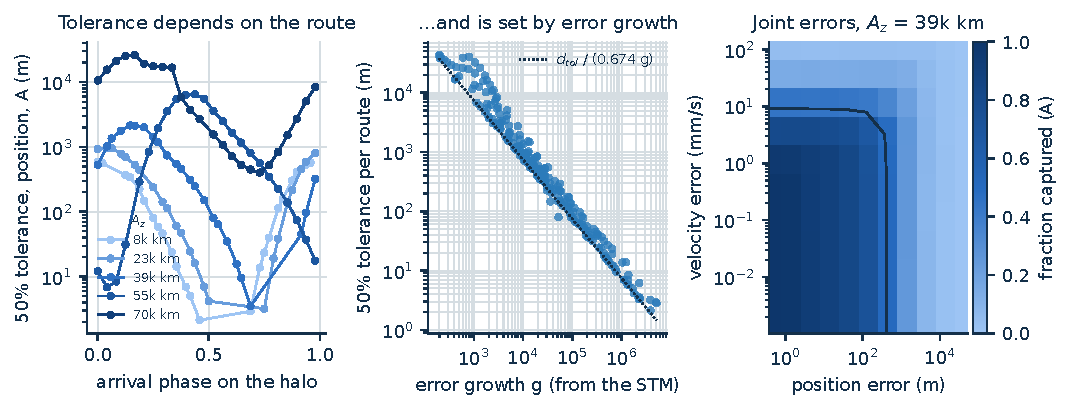
\includegraphics[width=\linewidth]{figures/fig7_routes_and_joint_errors.pdf}
\caption{Left: 50\% position tolerance (A) for each injection route, for alternate halos. Centre: every route of every halo
against its linear error-growth factor; dotted: Eq.~\eqref{eq:lin}. Right: capture fraction for joint position and
velocity errors for one halo; the line is the 50\% contour.}\label{fig:route}
\end{figure}

\subsection{Relativity}\label{sec:rel}
Along the halos the 1PN acceleration is \(\PNRatioMed\) of the Newtonian gravitational acceleration (median; Fig.~\ref{fig:rel}, left),
consistent with the estimate $GM_\oplus/(rc^2)\sim10^{-11}$ once the velocity-dependent terms of similar size are included.
Three measurements show it does not affect the question asked here.
(i) The capture curves with and without the term coincide: the largest difference in any capture fraction is \(\PNMaxDiff\).
(ii) With identical random draws, \PNFlips\ of \PNTotal\ outcome classifications differ (position and velocity experiments, both definitions).
(iii) Flown from the same injection state, the 1PN trajectory departs from the Newtonian one by a median of \PNShiftMed~m (maximum \PNShiftMax~m)
by the end of the first revolution on the halo. That gap is the instability amplifying a tiny push; expressed as the injection
position error that would produce it, it is \PNEquivMedMM~mm (median) and at most \PNEquivMaxMM~mm, never more than \(\PNEquivOverTol\) of the
tolerance of the same route.
So, to the precision of this experiment, relativistic corrections do not change the capture tolerance; and a real design would
simply include the term in the nominal trajectory, removing even that offset.

\begin{figure}[t]\centering
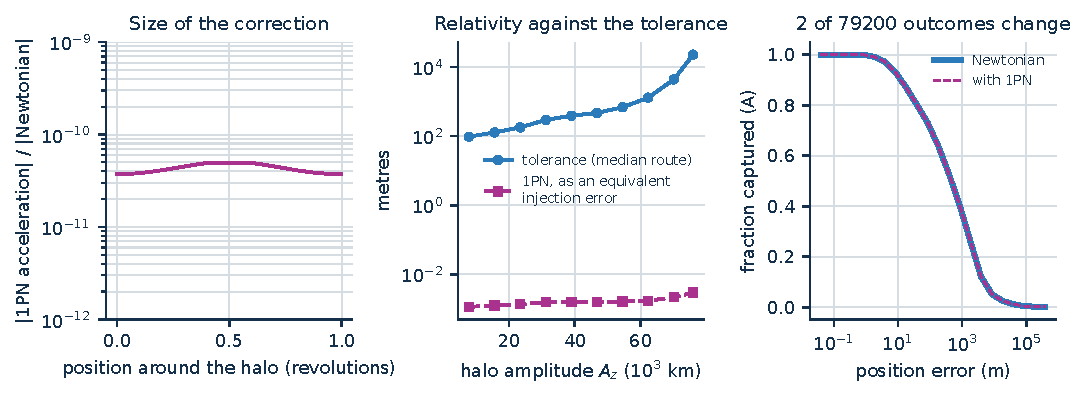
\includegraphics[width=\linewidth]{figures/fig8_relativity.pdf}
\caption{Left: ratio of 1PN to Newtonian acceleration around one halo. Centre: per-route tolerance (median over routes) against
the injection error equivalent to the 1PN effect. Right: capture curves with and without the 1PN term for one halo (they coincide).}\label{fig:rel}
\end{figure}

\subsection{Robustness}\label{sec:robust}
Table~\ref{tab:rob} repeats the position experiment for three halos with (a) every integration tolerance and the
step cap halved, (b) a different random seed, (c) the manifold displacement $\epsilon$ ten times smaller, and (d) the capture
tube half and twice as wide. Halving the tolerances changes at most a fraction of a percent of individual outcomes and leaves
$\sigma_{50}$ unchanged to within a few percent. A different seed and a ten-times smaller $\epsilon$ (which selects different routes on the same tube) both move $\sigma_{50}$ by less than its bootstrap range.
Change (d) moves $\sigma_{50}$ roughly as $d_{\rm tol}^{2}$, not linearly: one factor comes from the tube width itself, and a second because a
narrower tube is entered later (the stable component must first decay further), by which time the unstable component has grown by the same factor,
since $\lambda_s=1/\lambda_u$. Equation~\eqref{eq:lin} contains both effects through $g(t_e+T)$. The tolerance is therefore defined relative to the chosen tube and
cannot be quoted independently of it.

\begin{table}[t]\centering\small
\caption{Robustness of the 50\% position tolerance (definition A), in metres. ``Changed'': individual outcomes that differ
when tolerances are halved.}\label{tab:rob}
\begin{tabular}{rrrrrrrr}\toprule
$z_0$ & baseline & halved & changed & other & $\epsilon/10$ & $d_{\rm tol}/2$ & $2d_{\rm tol}$\\
(km) & (range) & tolerances & & seed & & & \\\midrule
\RobustRows
\bottomrule\end{tabular}
\end{table}

Because route-to-route variation dominates, a second check uses \emph{every} usable route of a finer scan. Table~\ref{tab:dense}
gives the Monte Carlo tolerance with all usable routes of a 48-trajectory scan, for $\epsilon$ and $\epsilon/10$, beside the linear prediction;
and the dotted curves of Fig.~\ref{fig:scale} show the linear prediction over all usable routes of a 96-trajectory scan for 24 halos.

\begin{table}[t]\centering\small
\caption{All-routes check of the 50\% position tolerance (definition A), in metres, with bootstrap ranges.}\label{tab:dense}
\begin{tabular}{rrrrr}\toprule
$z_0$ (km) & routes & Monte Carlo, $\epsilon$ & Monte Carlo, $\epsilon/10$ & linear, $\epsilon$\\\midrule
\DenseRows
\bottomrule\end{tabular}
\end{table}

\subsection{A sampling pitfall, and its correction}\label{sec:pitfall}
A first version of this experiment displaced the orbit by a \emph{constant} $\epsilon$ at evenly spaced phases, the usual recipe for drawing
manifolds. Its robustness test failed: with $\epsilon/10$ the pooled $\sigma_{50}$ moved from 198 to 79~m, from 530 to 284~m and from 664 to 2480~m
for the three test halos, far outside the bootstrap ranges, although the section curve had moved by only $3\times10^{-5}$ of its size.
The reason is that a trajectory of the tube is identified by its Floquet label $\theta=\phi-\ln(\epsilon/|p(\phi)|)/\ln\lambda_s$ (mod 1). With constant $\epsilon$,
$\theta$ is not a uniform function of $\phi$, so the trajectories are sampled unevenly, and changing $\epsilon$ shifts the uneven pattern.
Since tolerance varies by orders of magnitude across trajectories, the pooled statistic changed; an apparent plateau in tolerance against
amplitude in that version was the same artefact. Displacing by $\epsilon|p(\phi)|/\max|p|$ makes $\theta=\phi+\text{const}$, and all results in this paper use it.
The constant-$\epsilon$ recipe remains adequate for \emph{drawing} a tube; it is not adequate for \emph{statistics} over a tube.

\section{Limitations}
The assumptions of Section~\ref{sec:model} bound what can be concluded. In particular: (1) absolute tolerances
would change in an ephemeris model with the Sun; only the scaling and the ordering of routes are expected to carry over,
and that expectation is itself untested here. (2) Injection is defined at one place, the Moon-plane crossing; injecting
earlier or later along the manifold changes the growth factor. (3) Routes that graze the Moon were excluded;
they exist and would lower pooled tolerances. (4) Only the northern L$_2$ family between \AzMin\ and \AzMax~km was sampled, with ten members;
the quoted exponents are empirical fits over that range, not laws. (5) Bootstrap ranges reflect sampling over
\NSamples\ draws and \NPhases\ routes, not model error. (6) The relativistic test keeps the primaries on a Newtonian circle
and is first order only; given the size of the effect, higher orders cannot matter here. (7) The analytic seed coefficients were checked
against an independent open-source implementation rather than the original article, and the 1PN energy integral
used as a diagnostic was validated numerically rather than against a primary source.

\section{Future work}
Repeat the experiment in an ephemeris model (Sun, eccentricity) to test whether the scaling survives; add a single
correction manoeuvre and ask how its timing trades against injection accuracy; use realistic, correlated injection covariances;
extend to the L$_1$ family and to near-rectilinear orbits, where $k\to1$ and the present definition of capture needs rethinking;
and optimise over routes, since the route was found to matter most.

\section{Conclusion}
In the Earth--Moon CR3BP an uncorrected spacecraft injected at the Moon plane on the stable manifold of an L$_2$ halo
is captured half the time, in the sense of holding the halo for one revolution, if its position error is about
\SposAFirst~m for the smallest halo studied, rising to \SposALastKm~km for the largest and least unstable, roughly as $k^{\FitPosA}$;
the corresponding velocity errors are \SvelAFirst--\SvelALast~mm/s. Merely staying near the Moon tolerates errors tens to hundreds of times larger. The tolerance
is set by linear error growth, varies by orders of magnitude between arrival routes, and is unaffected by first-order relativistic
corrections. Statistics over a manifold tube must sample its trajectories evenly; the usual constant-displacement recipe does not.

\section*{Reproducibility}\label{sec:repro}
\texttt{python scripts/reproduce\_all.py} reruns the Monte Carlo (fixed seed 20261010), the analysis, every figure, the
numbers quoted in this text, the verification report and this PDF. Software versions are pinned in \texttt{requirements.txt}.

\section*{Acknowledgement of assistance}
The simulation code, figures and the first draft of this text were produced with the help of an AI assistant
(Claude, Anthropic) working to my specification. I am responsible for the research question, for checking the
work, and for any errors. \emph{[Author: edit this statement to match your venue's rules before submitting.]}

\begin{thebibliography}{9}\small
\bibitem{koon} W.~S. Koon, M.~W. Lo, J.~E. Marsden, S.~D. Ross, \emph{Dynamical Systems, the Three-Body Problem and Space Mission Design},
 Marsden Books, 2011 (free online edition v1.3, 2022), ISBN 978-0-615-24095-4. Chapter~2 consulted.
\bibitem{szebehely} V.~Szebehely, \emph{Theory of Orbits: The Restricted Problem of Three Bodies}, Academic Press, 1967.
 [Standard reference; not consulted directly for this draft.]
\bibitem{richardson} D.~L. Richardson, Analytic construction of periodic orbits about the collinear points,
 \emph{Celestial Mechanics} \textbf{22} (1980) 241--253, doi:10.1007/BF01229511. [Abstract consulted; coefficients cross-checked against the Orekit library.]
\bibitem{howell} K.~C. Howell, Three-dimensional, periodic, `halo' orbits, \emph{Celestial Mechanics} \textbf{32} (1984) 53--71,
 doi:10.1007/BF01358403. [Abstract consulted.]
\bibitem{jplapi} NASA/JPL Solar System Dynamics, Three-Body Periodic Orbits API, version 1.0,
 \url{https://ssd-api.jpl.nasa.gov/doc/periodic_orbits.html}, accessed 10 October 2026.
\bibitem{eih} A.~Einstein, L.~Infeld, B.~Hoffmann, The gravitational equations and the problem of motion,
 \emph{Annals of Mathematics} \textbf{39} (1938) 65--100, doi:10.2307/1968714. [Not consulted directly.]
\bibitem{assist} M.~J. Holman et al., ASSIST: an ephemeris-quality test particle integrator, arXiv:2303.16246 (2023), Eq.~(2).
\bibitem{ashby} N.~Ashby, Relativity in the Global Positioning System, \emph{Living Reviews in Relativity} \textbf{6} (2003) 1,
 doi:10.12942/lrr-2003-1, Eq.~(35).
\end{thebibliography}
\end{document}
